\begin{figure}[H]
	\centering
	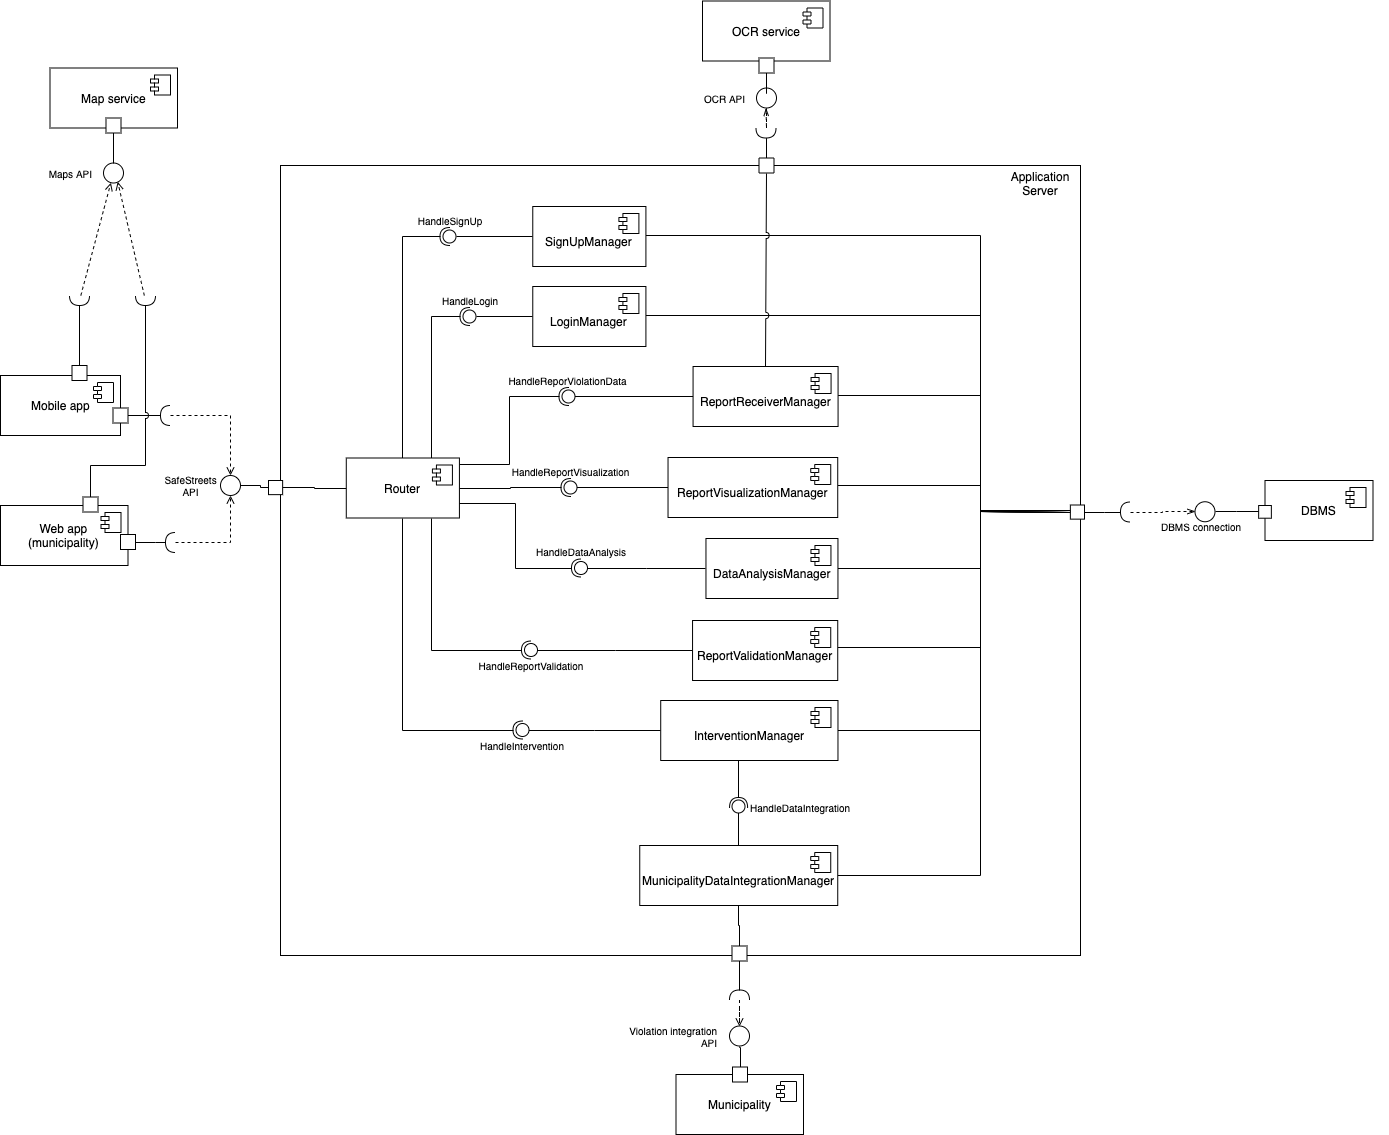
\includegraphics[width=.98\linewidth]{componentsDiagram.png}
	\caption{Components diagram.}
\end{figure}

Customers app subsystems (clients):
\begin{itemize}
	\item MobileApp (citizen/authorities)
	\item WebApp (municipality)
\end{itemize}

\subsubsection{Interfaces summary}
In the following, a list of all the system's interfaces subdivided into relevant categories is provided:\\

External interfaces:
\begin{itemize}
	\item DBMS
	\item Maps API
	\item OCR API
	\item Violation integration API
\end{itemize}

\bigskip
Router Interfaces accessible from mobile app:
\begin{itemize}
	\item HandleSignUp
	\item HandleLogin
	\item HandleReportViolationData
	\item HandleReportVisualization
	\item HandleDataAnalysis
	\item HandleReportValidation
\end{itemize}

\bigskip
Router interfaces accessible from municipality web app:
\begin{itemize}
	\item HandleSignUp
	\item HandleLogin
	\item HandleDataAnalysis
	\item HandleIntervention
\end{itemize}

\bigskip
\subsubsection{Component descriptions}
In this section, every internal component of the application server is analyzed and described in detail:

\begin{itemize}
	\item \textbf{Router:} 
	it listens for all requests made by clients on the SafeStreets API endpoint and provides handlers for each type of request. The handlers call various managers internal to the application server that are pertinent to the request made by the client, so that the router can receive from them the result of the operation and send back to the user a response.
	\item \textbf{SignUpManager:}
	module with the goal of handling registration requests of all user types. It checks that no data is missing and its correctness, by checking if the email has already been registered and if the password satisfy the given rules (e.g. at least 8 characters, at least 1 alphabetical symbol and 1 number, ecc...) and it's correctly repeated in the "repeat password" field. In case of authorities and municipalities account registrations, this manager also check that the provided PEC address domain matches one of the registered domains in the SafeStreets system: if the domain is present, the account is associated to the organization with that domain, otherwise the component returns an error to the user, telling it that the domain is not registered. If data provided by the registration is valid, then the manager registers the account by inserting it into the main database and returns a confirmation to the router, otherwise it returns an error.
	\item \textbf{OrganizationRegistrationManager:}
	module that can only be accessed by admins through an apposite interface, which details remain secret for security reasons. When a public institution request is approved, SafeStreets admins can register the organization data along with its PEC domain, so that its officers can register to the system. This component accepts only data sent by an admin account, checking also that no data is missing before inserting it in the database.
	\item \textbf{LoginManager:}
	module that handles login requests made by clients. It checks that email and password provided by the user in the login form is actually associated to an account registered in the database. If login is successful, a session package installed in the server will register the session, so that other components can check easily which account made the request and discriminate services and accessible data for each account type. This module returns a confirmation to the router module if login is successful, otherwise it returns an error.
	\item \textbf{ReportReceiverManager:}
	module that allows the correct registration of the reports data generated by the citizens and also the communication with the OCR service, used to recognize correctly the license plates from the first photo of the report. When a citizen starts the report generation procedure, it will be asked to take pictures of the violations, in which is stated that the first one should have the license plate of the vehicle involved in the violation clearly visible. After the citizen takes the pictures, the first one is sent to the server and then is passed to this manager responsible for sending a request to the OCR service to recognize the license plate of the vehicle. After receiving the result, the manager forwards it to the router and it's sent back to the user for confirmation. The managers also handles the whole report data when the citizen submits it to the application server. If the report is incomplete because some data is missing, the manager reports the error to the router that then sends back it to the client, otherwise the manager completes it with some meta data like the timestamp, address obtained by reverse geocoding the GPS coordinates with the Maps service, the userID of the citizen, and 'pending' status. Then it stores the report in the database, returning an "ok" message.
	\item \textbf{ReportVisualizationManager:}
	module associated to single reports data requests or list of reports requests. It provides the possibility to query database for searching reports associated to a specific city, or to a specific user, or a single report given its id. This covers all the requirements regarding specific report visualization that the users can make with the mobile apps. In fact, authorities can access a list of all reports that are related to their city and a citizen instead can access the list of all reports made by himself; both type of users can then select a report from the list and send a request to the router module with the report id attached. It's important that the ReportVisualizationManager checks what type of account made the request from the session, so that it can check whether the request is valid or fraudulent in order to avoid the possibility of not authorized data access. 
	\item \textbf{ReportValidationManager:}
	module that permits a report validation or invalidation made by authorities. It associates the authority ID to the report and changes the status of the report according to the one selected by the supervisor. Obviously the changes are made directly on the database, updating the record with the ID of the report present in the request. Also here is checked that the report that is going to be modified is actually accessible from the authority that made the request (it's situated in the city in which the authority has jurisdiction, that is retrievable from the database).
	\item \textbf{DataAnalysisManager:}
	module that handles the requests for data analysis, that involve the representation of data from multiple reports that match the filters specified by the client. Every request received by this component contains temporal filters (from what date and to which date), spatial filters (the interested city) and violation type filter, that are then used by the manager to query the database and return to client all the validated reports data that satisfy the filters. Note that like ReportVisualizationManager, also this component need to check which type of account made the request and filter some data based on its permissions. If the request is made by a citizen account, the license plates, the submitter data and the supervisor (authority that validated the report) are omitted from reports' data, to avoid common citizen to visualize sensible data that is also not relevant for their analysis; instead if the request is made by authorities and municipalities' accounts, they can visualize all data associated to the reports. Another consideration is that the server only provides the data to clients but doesn't define or bind the method to visualize this data in any way.   
	\item \textbf{InterventionManager:}
	module that handles municipalities' requests for generating new lists of possible interventions, targeted to provide possible solutions to the frequent violations in the most unsafe areas of their cities. Before generating the interventions, this module calls the MunicipalityDataIntegrationManager to integrate municipality's data in the SafeStreets' database, if possible. After receiving a response from the MunicipalityDataIntegrationManager, the list of interventions will be generated. An algorithm consults all the reports present in SafeStreets database that are located in the city of the municipality that made the request, and checks for the areas with the highest density of violations. After computing the most unsafe areas of the city, the algorithm checks the type of violations recurring for each single area and from that it computes all possible interventions that can solve the problem. When all the process is finished, the result is returned to the router, in combination of a possible error raised from the MunicipalityDataIntegrationManager so that the user is aware of the fact that data integration was not possible and he could investigate the problem.
	\item \textbf{MunicipalityDataIntegrationManager:}
	module that allows the integration of violation data from any municipality API structured according to SafeStreets reference API model. It is accessed by the InterventionManager when a municipality requests the generation of a list of possible interventions to do in its territory. The module checks if the municipality that made the request has provided an API for accessing its data, if present in the database it requests all violation data that have a date later than the one indicated in last intervention generation timestamp (gets all data if no intervention generation was made by the municipality in the past), and integrate it in SafeStreets database. When the process is done, the manager notifies the InterventionManager, that is waiting a response from it before initiating the intervention generation. Note that if no API is associated to the municipality the integration will be immediately aborted, instead if the municipality's API endpoints or its provided data have not the structure expected (not compliant with the reference model) the MunicipalityDataIntegrationManager will return an error to the InterventionManager, that will continue without the municipality's data integration, using only data contained in SafeStreets' database (the error is reported to the user in this case).
\end{itemize}


\subsubsection{Entity-relationship diagram}
The entity-relationship diagram below describes the conceptual model of the database.

\begin{figure}[H]
	\centering
	\includegraphics[width=\linewidth]{Images/ER_diagram.png}
	\caption{Entity-relationship diagram.}
\end{figure}

In comparison with the class diagram presented in RASD document, the main entities user, report and intervention have UserID, ReportID, and InterventionID primary key attributes, respectively, that are used for a faster lookup on the database. In fact using strings or multiple fields primary keys are not advisable in case performances are concerned, because indexing them is more difficulty and require more database block lookups compared on indexing on a single int number. Also, the IDs guarantees the uniqueness of the primary key in case that a table doesn't have any relevant unique identifier among its fields.

